\chapter{Day 1: shapes, colors \& variables}

\section{Summary of topics}
% Summarize the topics from the “listen” segment of the day (150 – 250 words)
During this lecture the layout of the PDE was explained. A basic program to draw a line was shown. Here, it was showed that one can draw basic shapes in processing using a variety of functions. These functions have a number of parameters. These are things like numbers, strings or booleans that change the behavior of the function. Examples are:

\begin{codebox}{Example 1.1}
    \begin{lstlisting}
println("Hello"); // print "Hello" in the console
size(400, 400); // set the screen size to 400 by 400 pixels
point(50, 90); // draw a point at x = 50, y = 90
    \end{lstlisting}
\end{codebox}

It was also explained that by using two slashes, you can create comments, which help explain code to others (like I did above). Furthermore, the coordinate system of the screen (going from left to right and from above to below) and the drawing order was shown. Colors of objects can be changed, by using:

\begin{codebox}{Example 1.2}
    \begin{lstlisting}
fill(255, 0, 0); // set the fill color to red
background(0, 255, 0); // set the background to green
stroke(0, 0, 255, 127); // set the stroke color to translucent blue
    \end{lstlisting}
\end{codebox}

The 4 parameters representing the R, G, B and Alpha values.

Next, variables where explained. These are small pieces of data that can represent numbers, letters, words, colors booleans etc. They are created using a type specifier like \texttt{int} or \texttt{boolean} followed by a name. Naming variables is done using camelCase. One can then use this name to assign data to the variable and then use the variable like:

\begin{codebox}{Example 1.3}
    \begin{lstlisting}
int a = 20; // declare a variable a and assign 20 to it
point(a, a); // use a to place a point at 20, 20
    \end{lstlisting}
\end{codebox}

Processing also has build-in variables, like \texttt{width} and \texttt{height}.

Then, some basic mathematics where shown. You can add values or variables together using ``+'', subtract them using ``-'', multiply using ``*'' and divide using ``/''. It is important to keep track of the data types when doing this. It is also possible to change the datatype. For example, changing a value to an integer is possible using \texttt{int().}

Finally the \texttt{random()} function was explained. It returns a float between 0 and the given number or when two numbers are given, between the two numbers, like this:

\begin{codebox}{Example 1.4}
    \begin{lstlisting}
float randomNumber = random(20); // return a random float from 0-20
int randomNumber = int(random(5, 20)); // return a random int from 5-19
    \end{lstlisting}
\end{codebox}

\section{Challenge description: Half-tone}
% A description of that day’s challenge describing what the assignment was, what you tried to achieve and how you applied the topics from the “listen” segment. include instruction on how to use is and Include screenshots/screen captures. (150 – 250 words)

The goal of the assignment was to create a static artwork which is different, yet similar every time you run the program. My goal was to create a half-tone image. Half-tones are images consisting of little dots of various sizes, traditionally used in printing. The larger the dots, the darker that part of the image appears, creating a shading effect, as can be seen in \cref{fig: half-tone}.

\begin{figure}[H]
    \centering
    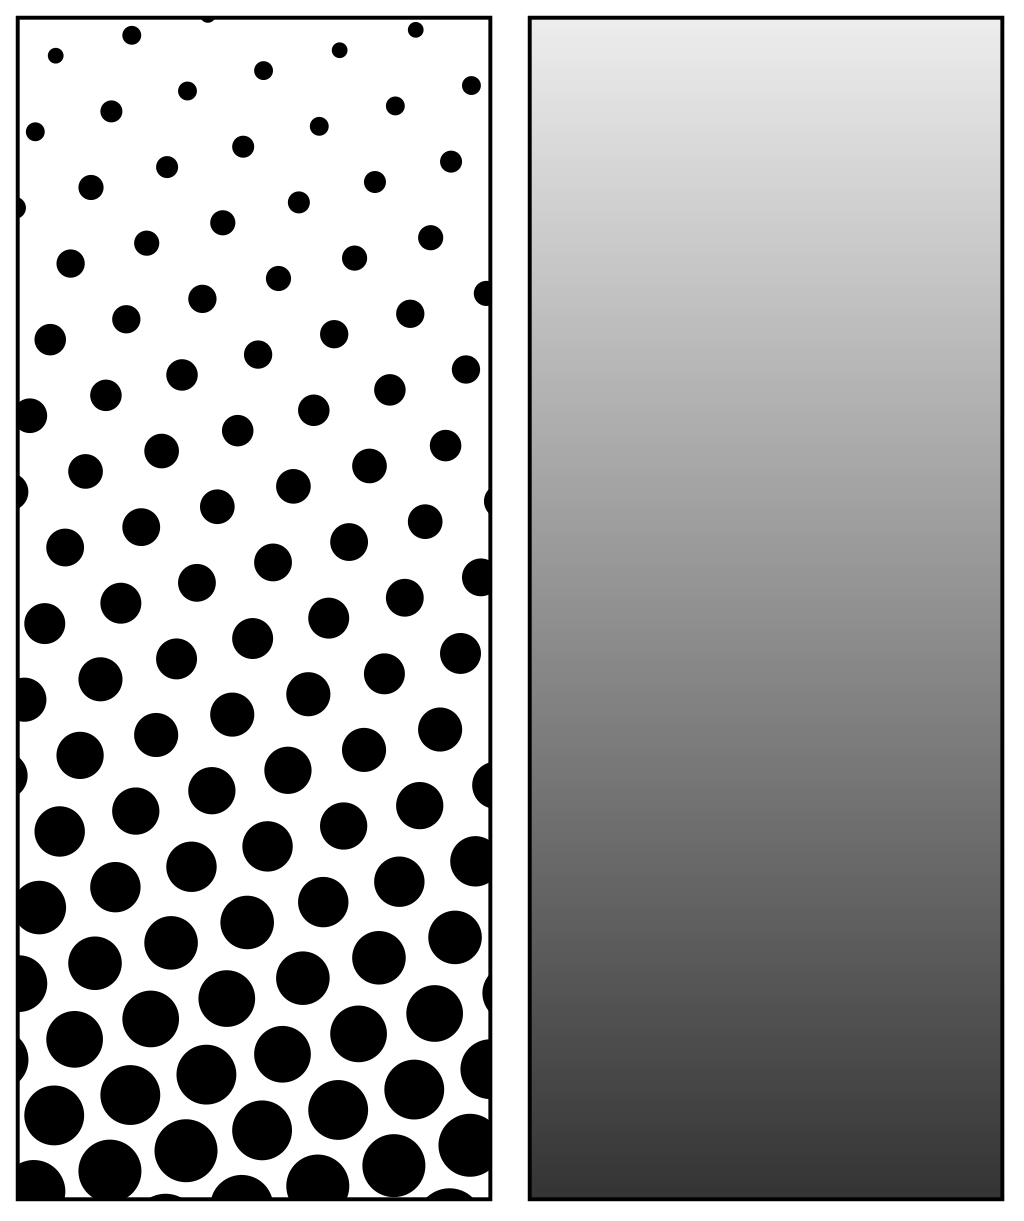
\includegraphics[width = 5cm]{Figures/day_1/half_tone.png}
    \caption{Half-tone (left) compared to the desired effect (right)}
    \label{fig: half-tone}
\end{figure}

In the code, I load in multiple pieces of art and pick a random one that will be converted into a halftone. I also randomize the color of the dots using the \texttt{fill()} and \texttt{random()} functions. Throughout the program I use variables to store the image data and color values of a specific pixels in order to determine the size of the dots. I finally use the \texttt{ellipse()} function to draw the dots and achieve the effect.

The user can restart the application to get a new random image and dot color. I have included a total of se artworks which are displayed in \cref{fig: half-tone art}.

\begin{figure}[H]
    \centering
    \begin{subfigure}[b]{0.45\textwidth}
        \centering
        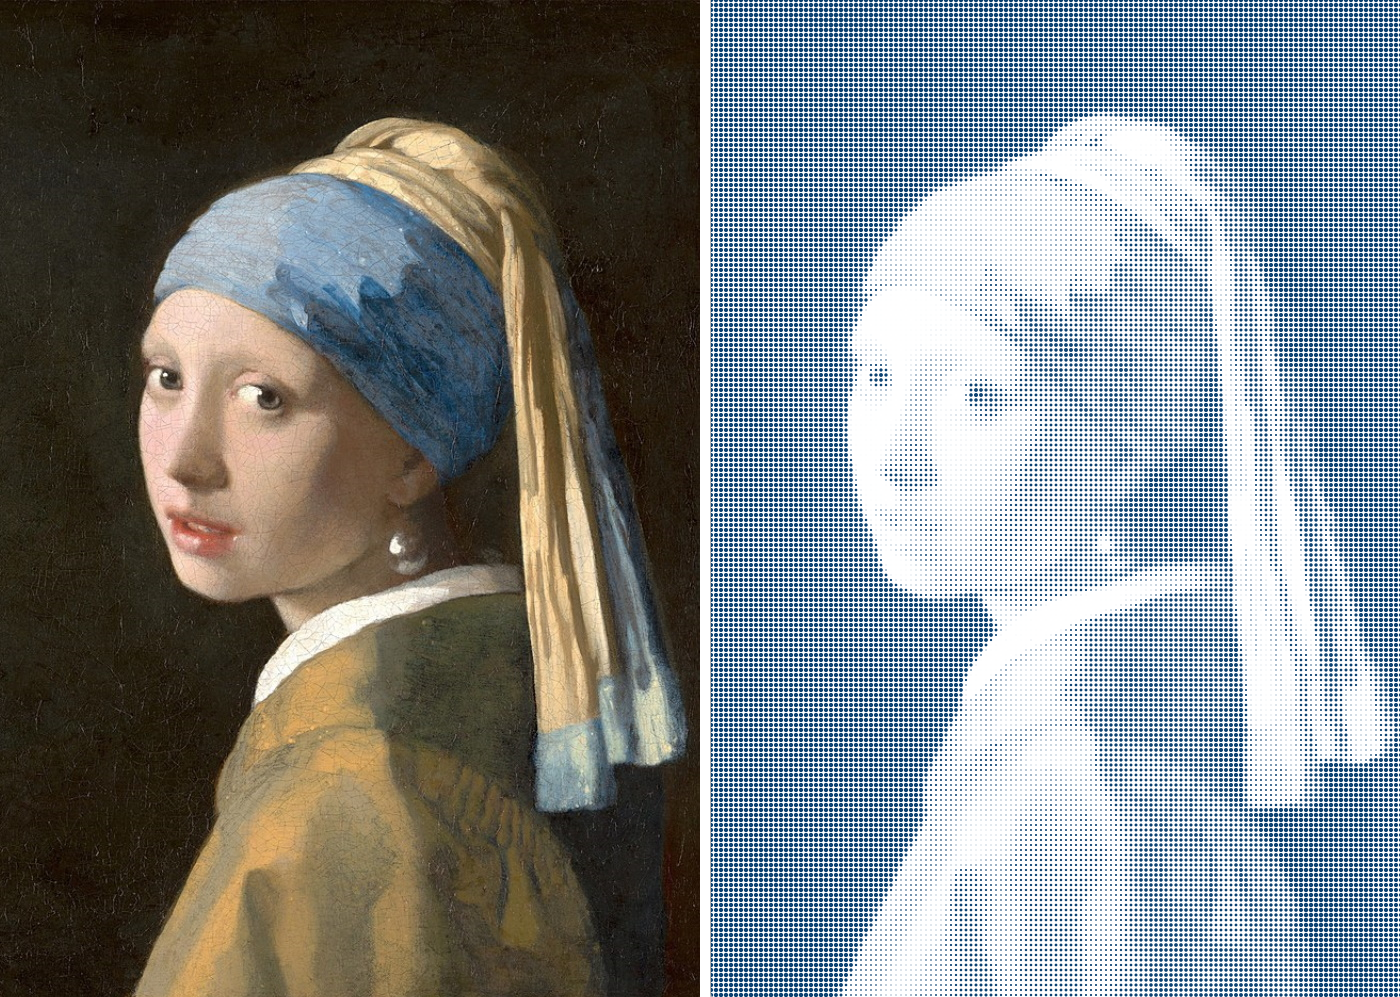
\includegraphics[width=\textwidth]{Figures/day_1/girl_with_the_pearl.png}
        \caption{Johannes Vermeer - Girl with a Pearl Earring}
    \end{subfigure}
    \hspace{1cm}
    \begin{subfigure}[b]{0.45\textwidth}
        \centering

        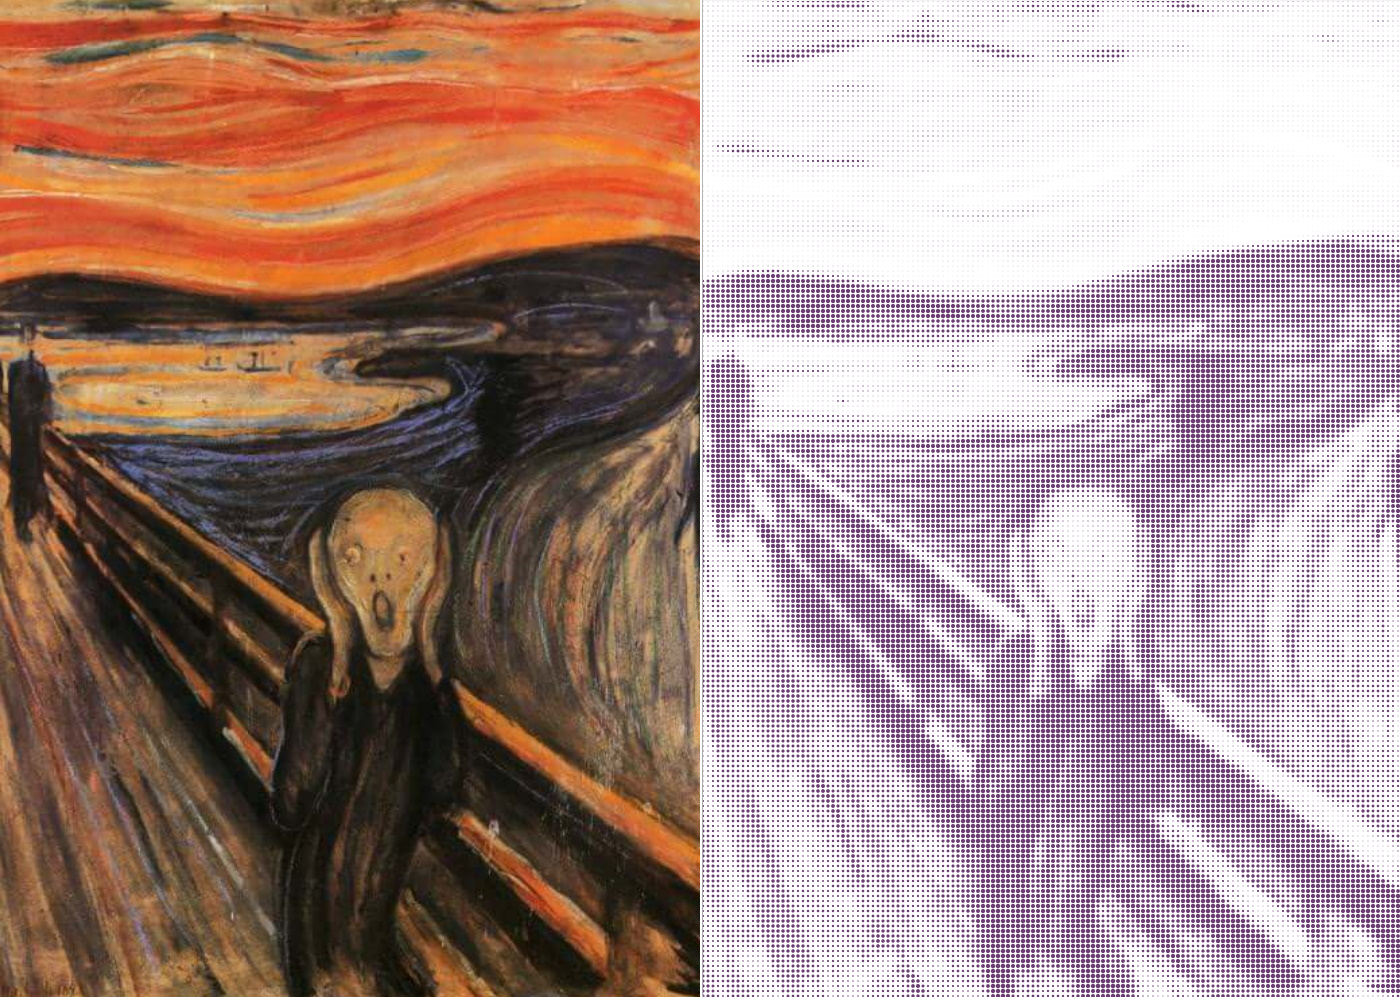
\includegraphics[width=\textwidth]{Figures/day_1/the_scream.png}
        \caption{Edvard Munch - The Scream}
    \end{subfigure}

    \begin{subfigure}[b]{0.45\textwidth}
        \centering
        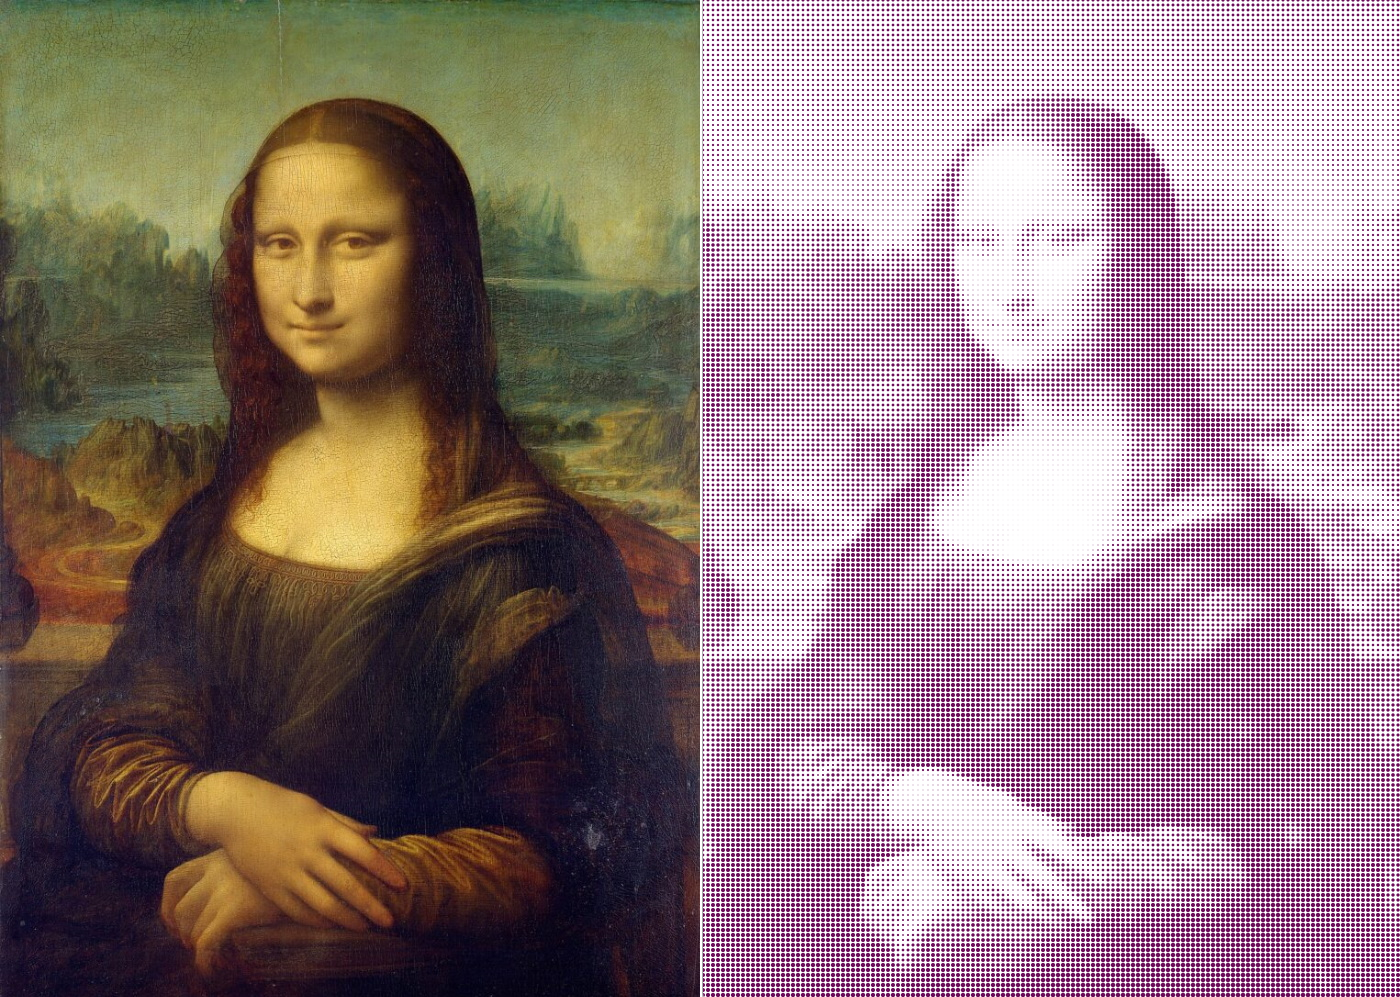
\includegraphics[width=\textwidth]{Figures/day_1/mona_lisa.png}
        \caption{Leonardo da Vinci - Mona Lisa}
    \end{subfigure}
    \hspace{1cm}
    \begin{subfigure}[b]{0.45\textwidth}
        \centering

        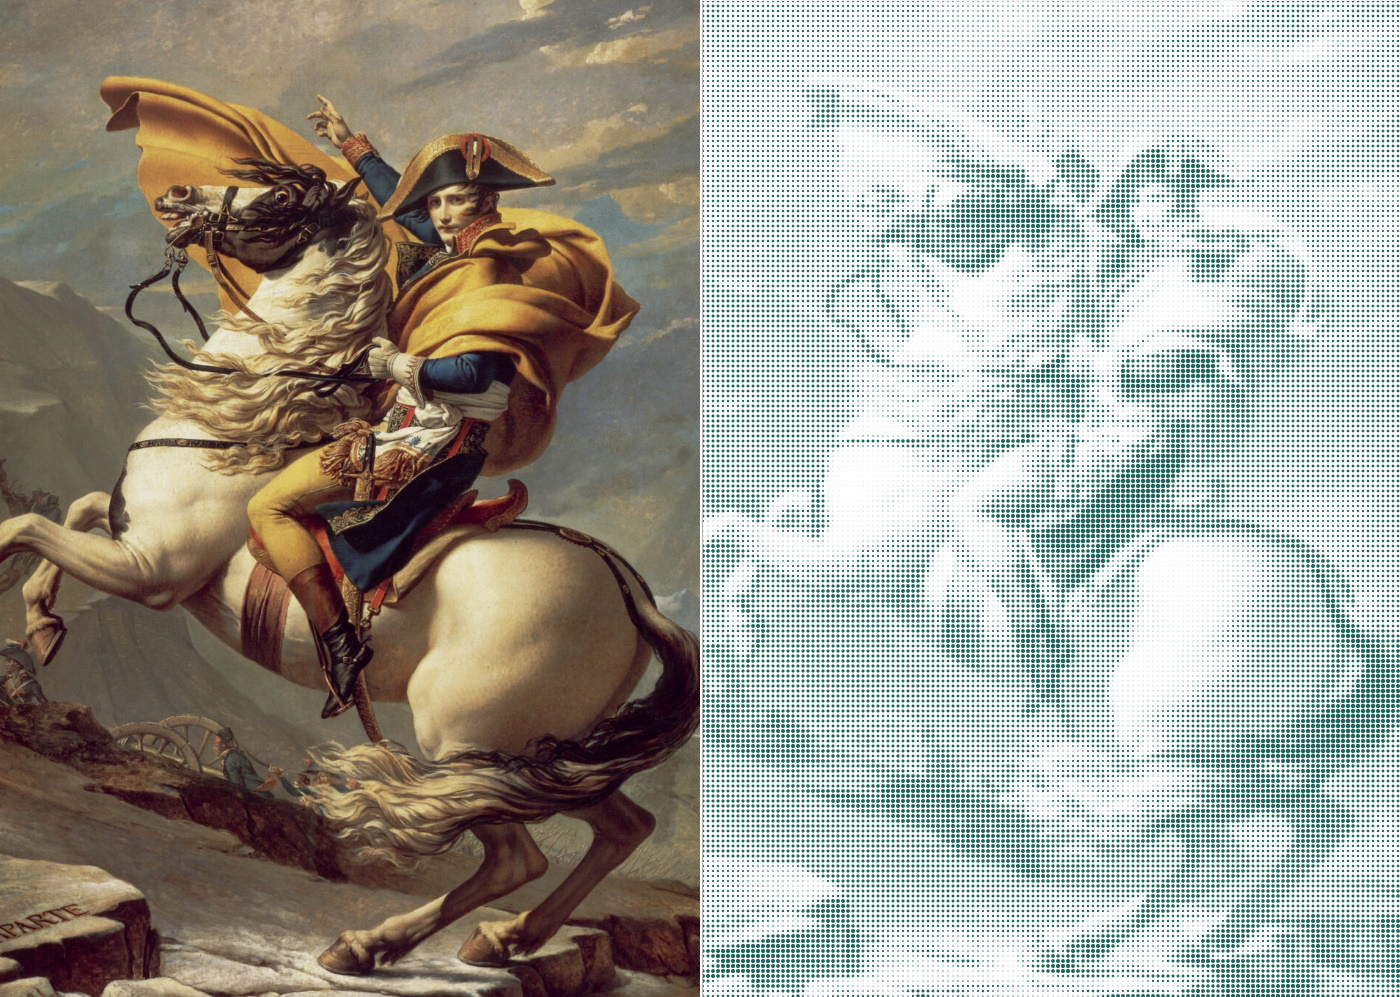
\includegraphics[width=\textwidth]{Figures/day_1/napoleon.png}
        \caption{Jacques David - Napoleon Crossing The Alps}
    \end{subfigure}

    \begin{subfigure}[b]{0.45\textwidth}
        \centering
        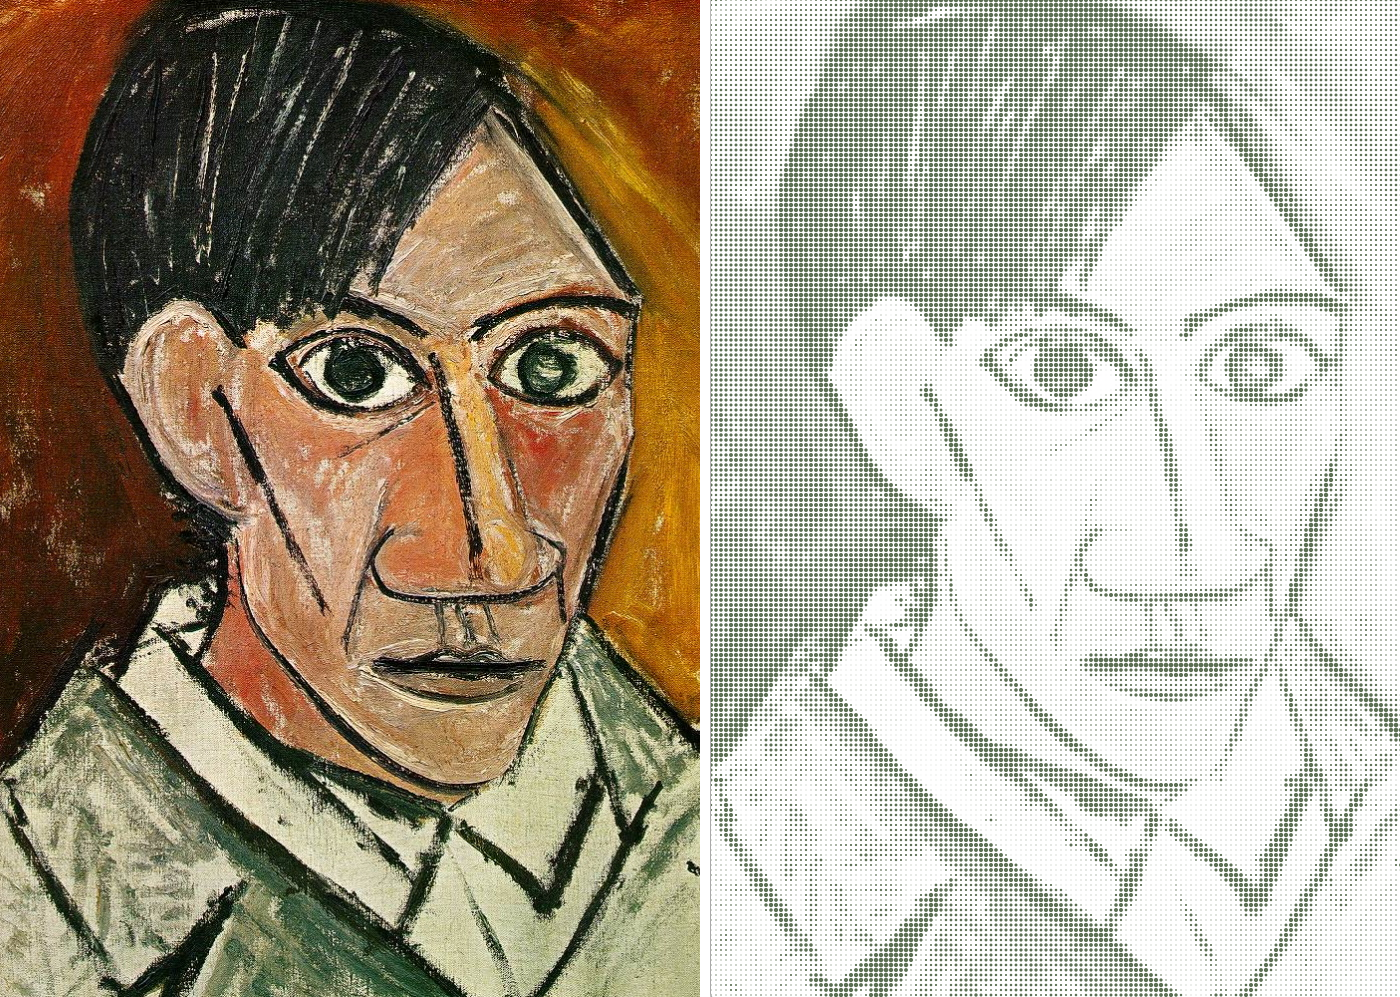
\includegraphics[width=\textwidth]{Figures/day_1/picasso.png}
        \caption{Pablo Picasso - Autoritratto}
    \end{subfigure}
    \hspace{1cm}
    \begin{subfigure}[b]{0.45\textwidth}
        \centering

        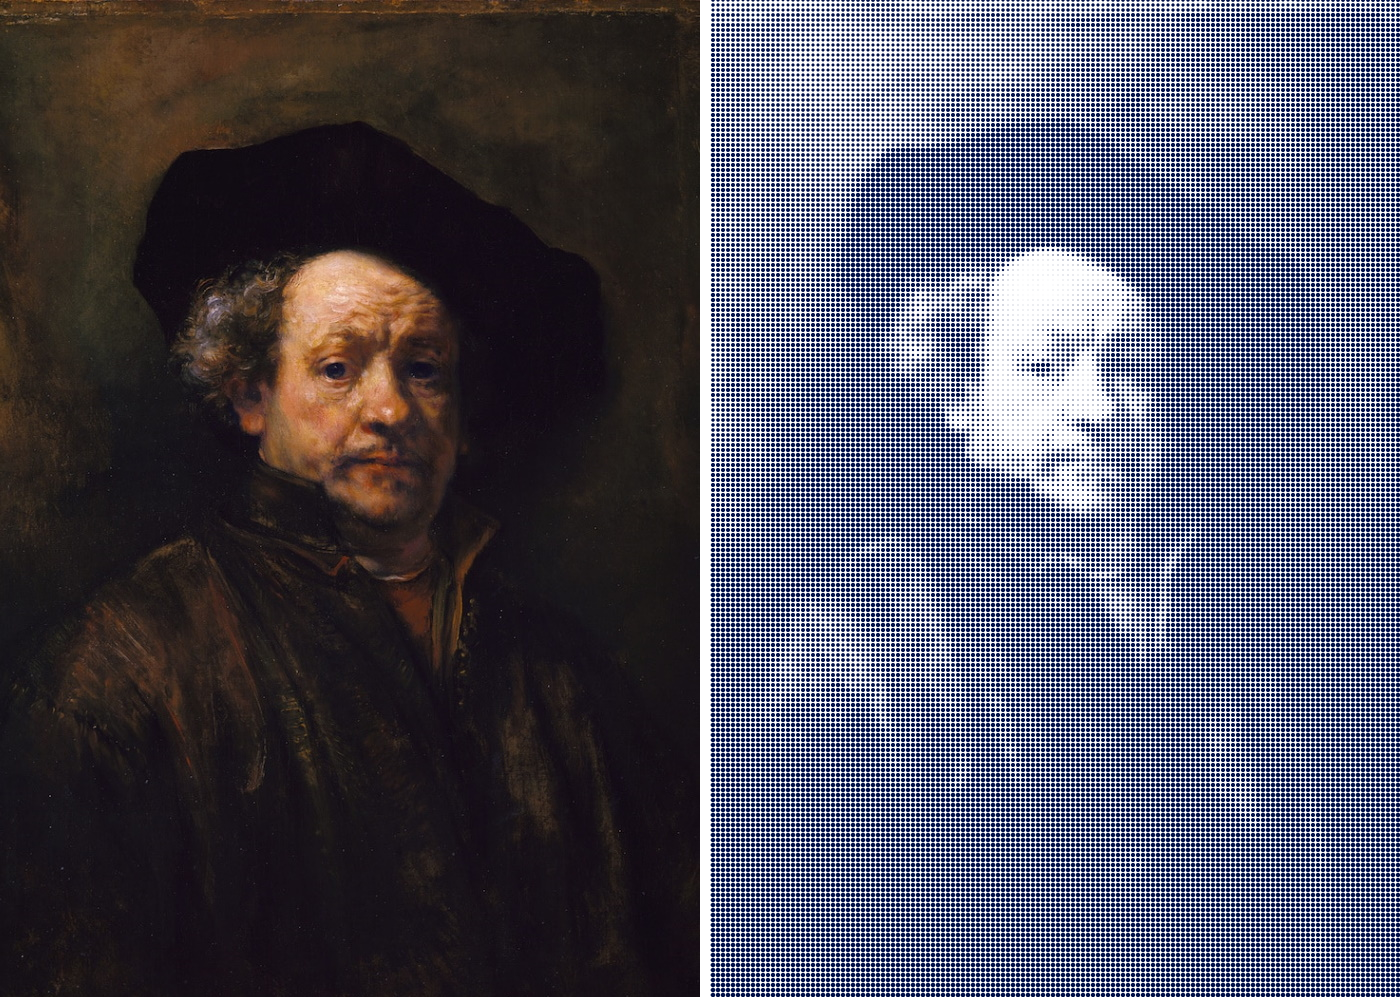
\includegraphics[width=\textwidth]{Figures/day_1/rembrandt.png}
        \caption{Rembrandt van Rijn - self portrait}
    \end{subfigure}

    \begin{subfigure}[b]{0.45\textwidth}
        \centering
        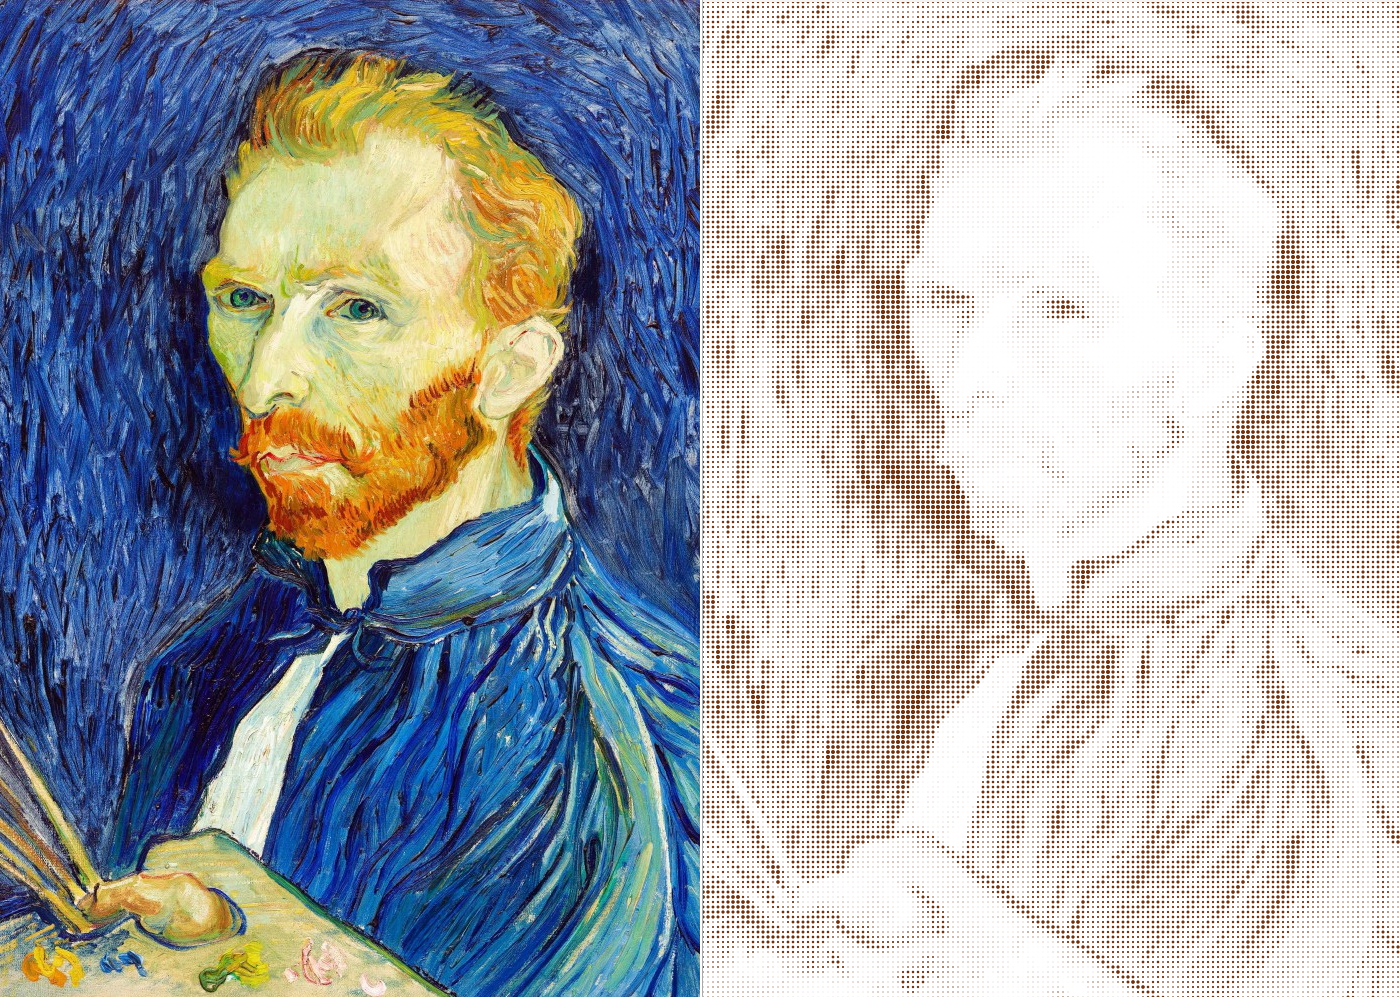
\includegraphics[width=\textwidth]{Figures/day_1/van_gogh.png}
        \caption{Vincent van Gogh - self portrait}
    \end{subfigure}

    \caption{Seven famous artworks as half-tones}
    \label{fig: half-tone art}

\end{figure}